\section{Line Fitting}

\subsection{Least Square Method}

\begin{figure}[htbp]
    \centering
    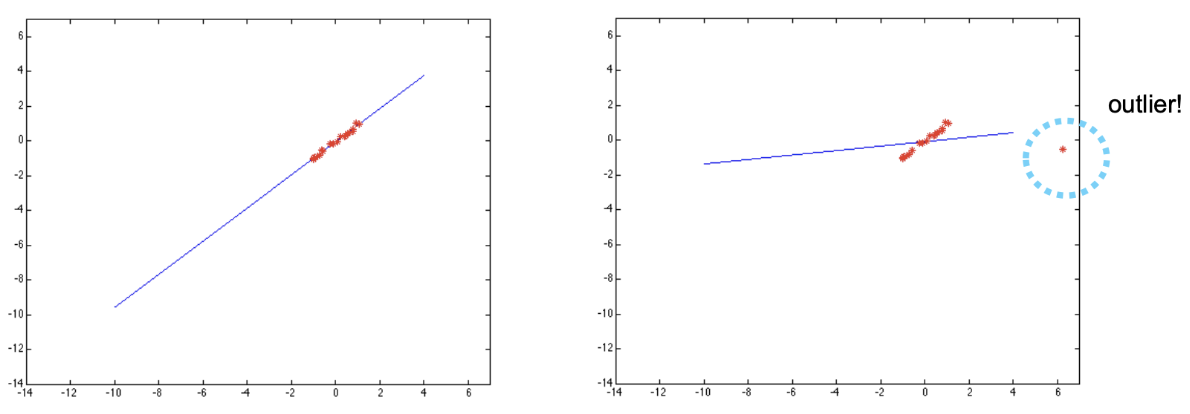
\includegraphics[width=0.8\textwidth]{figures/not_roboust_outliner.png}
    \caption{Least Square Method is not robust to outliers}
\end{figure}

Robust to small noises but sensitive to outliers.

\subsection{RANSAC}

RANSAC:RANdom SAmple Consensus

Idea: we need to find a line that has the largest supporters (or inliers)

RANSAC loop:

假设这个直线 (平面) 需要两个 (n个) 点来确定.

\begin{enumerate}
    \item 随机选择 k 组能确定这个直线的点,也就是在所有点里面选出一个 $k\times 2$ 的矩阵
    \item 对每一组点计算出一条直线
    \item 对每一组点的直线计算出所有点到这条直线的距离,如果小于阈值,则认为这个点是这条直线的 inlier
    \item 找到最大的 inlier 数量的直线,如果大于阈值,则认为这条直线是最优的
    \item 对这个最优的直线,用这个直线所有的 inlier 重新计算一次直线
\end{enumerate}

\subsection{RANSAC calculation}

假设我们有所有 inliner 占比为 $w$ 的先验知识,同时希望有不低于 $p$ 的概率能够找到一个最优的直线,那么我们需要多少次迭代呢?

\begin{equation}
\mathbf{\Pr}\text{[一组点全部是inliner]} = w^n
\end{equation}

如果一组点中有一个点是 outliner,那么我们称这组点 fail.

\begin{equation}
\mathbf{\Pr}\text{[k组点全部fail]} = {(1-w^n)}^k
\end{equation}

我们希望 k 组点全部 fail 的概率小于 $1-p$.

\begin{equation}
{(1-w^{n})}^k < 1-p
\Rightarrow
k > \frac{\log(1-p)}{\log(1-w^n)}
\end{equation}

\subsection{Hough Transform}

其实就是把一条直线从实际空间的表示转换到参数空间的表示.但是如果存在垂直的直线,可能需要考虑使用极坐标来作为参数空间.

\begin{figure}[htbp]
    \centering
    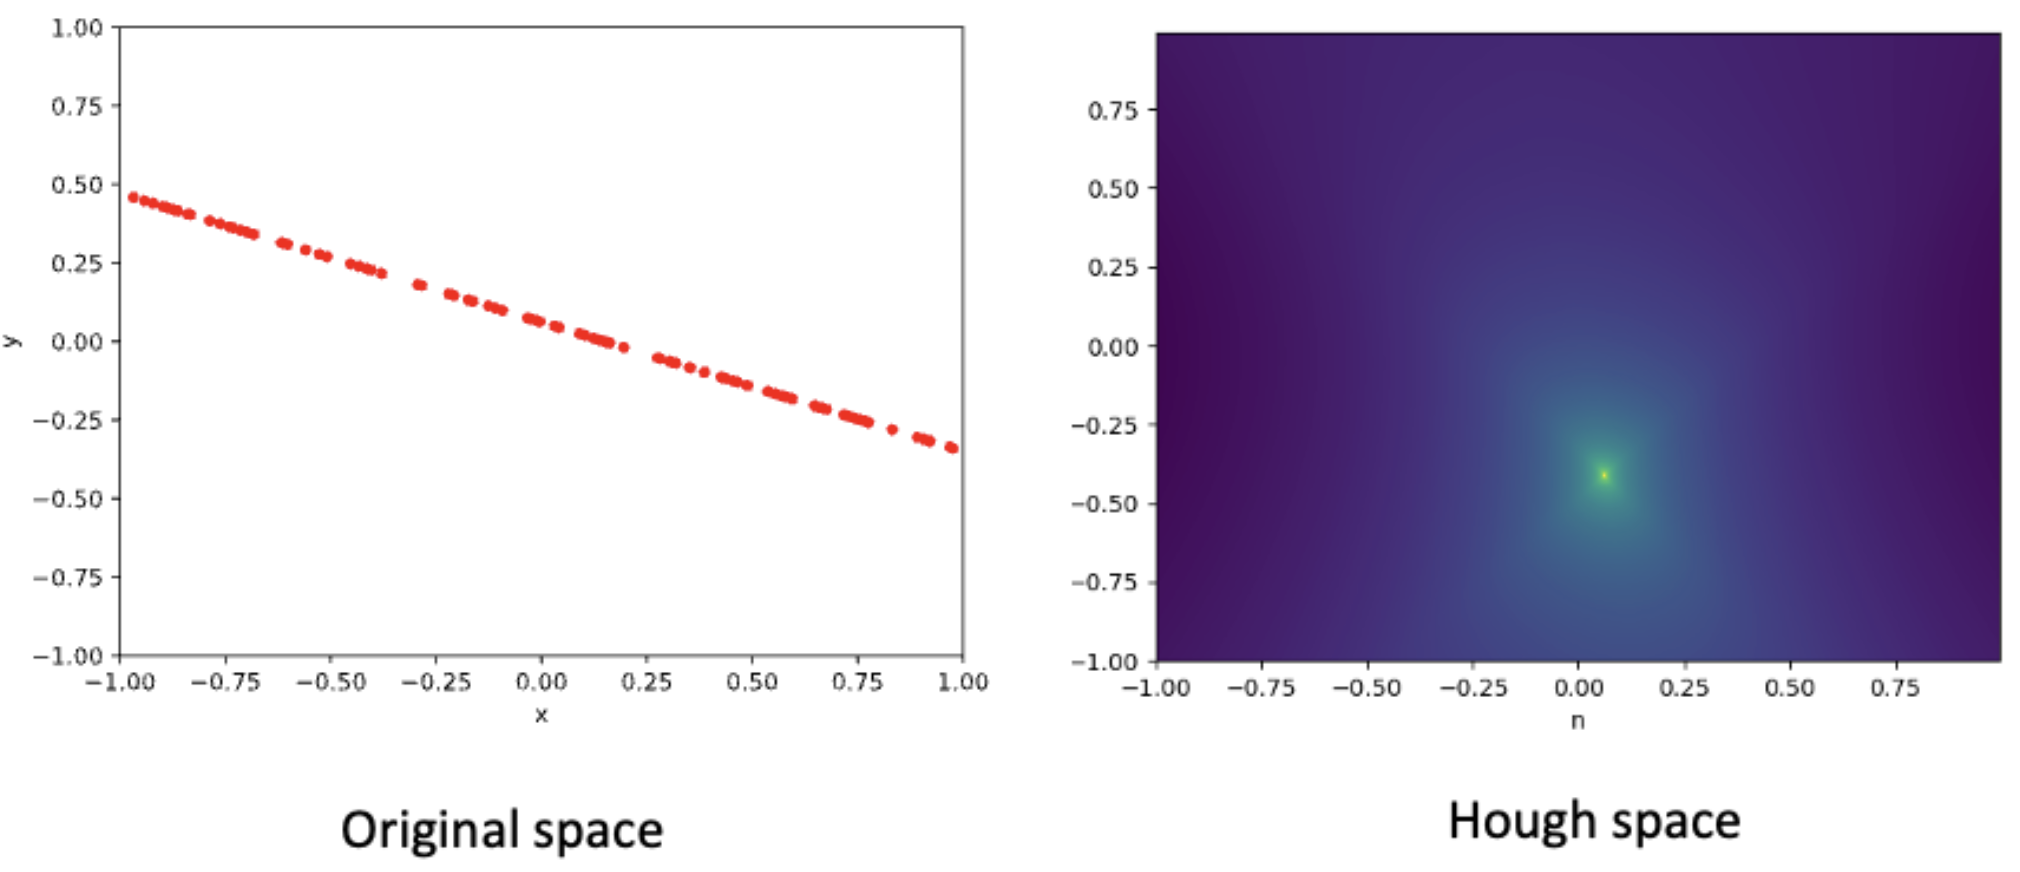
\includegraphics[width=0.8\textwidth]{figures/hough1.png}
    \caption{Hough Transform w/o Noise}
\end{figure}

\begin{figure}[htbp]
    \centering
    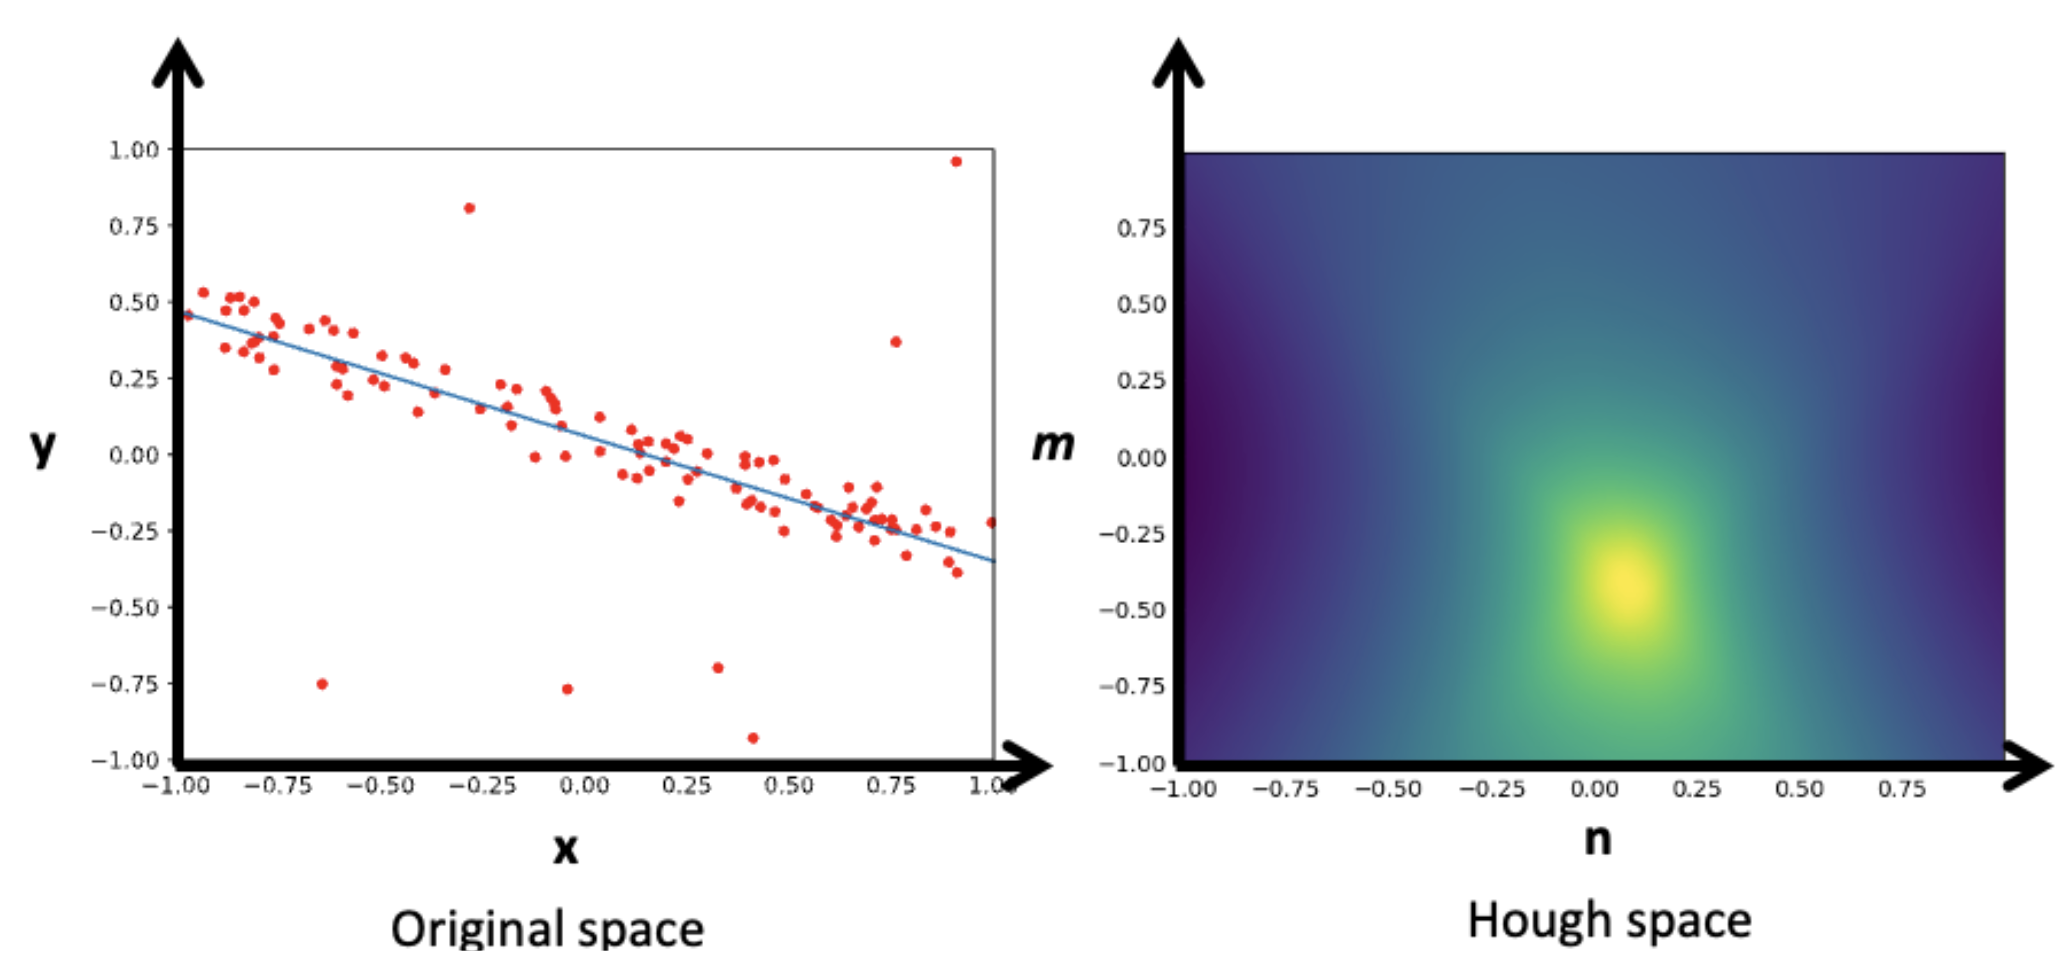
\includegraphics[width=0.8\textwidth]{figures/hough2.png}
    \caption{Hough Transform w/ Noise and Outliers}
\end{figure}